%&latex
%
\documentclass[../template.tex]{subfiles}
\usepackage{amsbsy}

\begin{document}

\section{Introduction} %computational physics
\lesson{1}{3/10/2019}
%Password moodle: NPhyS-2019.\\
%App Socrative Student. Course: Lenzinp.
The goal of this course is to introduce a series of problems in modern physics (in particular of statistical mechanics), describe their origin, the needed mathematical tools and their resolution. At the end of the lectures, one student should be able to formulate problems and solve them. Exercises will be published online, and the final exam will consist of a theoretical question and a problem to solve (similar to the ones seen during the course). It will be needed to bring an \textit{exercise book} with all the written solutions of the course's exercises.\\
%Goals and modality need to be known for the exam


\section{The Diffusion Process}
In classical mechanics, if we know all forces $\vec{F}$ that act on a certain particle, along with its initial condition (e.g. position $\vec{x}(t=0)$ and velocity $\vec{v}(t=0)$), we can compute its trajectory $\vec{x}(t)\> \forall t$ by integrating the equations of motion.\\
This is indeed true even for ensembles of particles - but it becomes very impractical for macroscopical objects. For example, a drop of water contains something in the order of $10^{23}$ molecules, and so to completely describe its motion it is needed to integrate six times that many equations ($3$ for position, $3$ for velocity for each single particle). Even if we had the computational capacity to do so, it would not be possible to know the necessary initial conditions with the required precision.\\

On the other hand, it is not very interesting to solve this kind of problem, because one could not possibly understand the intricacy of this motion, and so the task doesn't give much insight in the relevant physics. In fact, we are most interested in the \textit{macroscopical} properties of the object. For example, one could consider the \textit{diffusion problem} of describing what happens to a droplet of ink in water. Just knowing the chemical details of the ink, and some macroscopical quantities, in principle we should be able to tell something about the system's evolution.\\

There are many mathematical tools that are needed for such a problem - one example is that of the \textit{path integral}, which is common to many areas of physics (for example QM), and will be tackled in the next lectures.\\

Some of the relevant results for the diffusion problem are:
\begin{itemize}
\item Fick's Law ($\sim 1895$)
\item Einstein's paper on brownian motion ($1905$). This was especially relevant because it was the first demonstration of the discrete nature of matter. Einstein observed that a fine powder, not containing any \textit{living organisms}, moved erratically if suspended in still water. If we assume that water is composed of particles, the single grains of powder behave like large objects hit by smaller particles. The number of hits on each side is almost the same, so the total force which acts on the large object is almost $0$. However, if the grains are sufficiently small, the slight unbalance in the number of collisions is significant, and leads to a kind of \textit{random motion}.\\

For example, let's consider a spherical grain submerged in the liquid. Let's call $U$ the upper emisphere, and $L$ the lower one. Denote with $\bar{N}_c$ the average number of collisions per second per surface unit. Then the number of hits on $U$ is \textit{almost} the same to that of $L$, up to a certain error:
\begin{align*}
\bar{N}_c \cdot U = \bar{N}_c \cdot L \pm \sqrt{\bar{N}_c}
\end{align*}
Then, the relative error is $\sqrt{\bar{N}_c}/\bar{N}_c = 1/\sqrt{\bar{N}_c}$, and it is especially high if $\bar{N}_c$ is small, which is true if the target grains are small.
\end{itemize}

Let's start by considering a particle in a starting position $\vec{r}(t=0)=\vec{r}_0$.\\
More generally, we can describe the \textit{initial conditions} as the \textit{starting distribution}.
\begin{enumerate}
\item For a discrete, point particle we have $\rho(\vec{r},0)=\delta^3(\vec{r}-\vec{r}_0)$
\item For some quantity of matter (for example a droplet of ink), we have some uniform initial density:
\begin{align*}
\rho(\vec{r},0) = \rho_0(\vec{r}) = \begin{cases}
\bar{\rho}_0 & |\vec{r}|<R\\
0 & \text{otherwise}
\end{cases}
\end{align*}
In the following, $\rho(\vec{r},t)$ is taken as a probability density, and not as a usual density of matter. The difference is merely of normalization. If $N$ is the total number of particles in ink, then $N\rho(\vec{r},t)$ is the density of ink particles at \textit{the specific} position $\vec{r}$ and time $t$.\\
So, the following holds:
\begin{align*}
1 &= \int_V d^3r \rho(\vec{r},t)\\
N &= \int_V d^3r \underbrace{N\rho(\vec{r},t)}_{\text{density at $\vec{r}$}}
\end{align*}
The meaning of a point-wise density can be understood as a limit:
\begin{align*}
N \rho(\vec{r},t) = \text{density at $\vec{r}$, time $t$} = \lim_{\Delta V \downarrow 0} \frac{\Delta N}{\Delta V}
\end{align*}
Consider a patch of liquid of volume $\Delta V$, that contains a number $\Delta N$ of ink particles. By letting it shrink \q{enough}, $\Delta N/\Delta V$ reaches a constant value - that is the density in a macroscopically small patch of liquid. Of course, $\Delta V$ cannot reach $0$, because in that case $\Delta N = 0$. So, the limit is to be interpreted in a macroscopical sense ($\Delta V$ is macroscopically vanishing, $\Delta V \downarrow 0$) and not in a mathematical sense ($\Delta V \to 0$).

\begin{minipage}[t]{0.45\textwidth}
\begin{figure}[H]
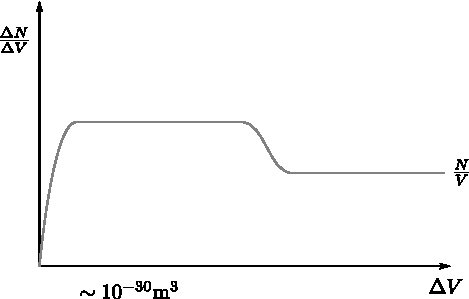
\includegraphics[width=\textwidth]{Plots/patch_centered_ink.pdf}
\caption{Density (ratio $\Delta N/\Delta V$) as function of patch size $\Delta V$ for a regio centered around the ink distribution $\rho_0$ ($|\vec{r}|<R$ at $t=0$). If $\Delta V$ is sufficiently large, the patch comprises also some space without ink, and so the density is lower.}
\end{figure}
\end{minipage}\hfill%
\begin{minipage}[t]{0.45\textwidth}
\begin{figure}[H]
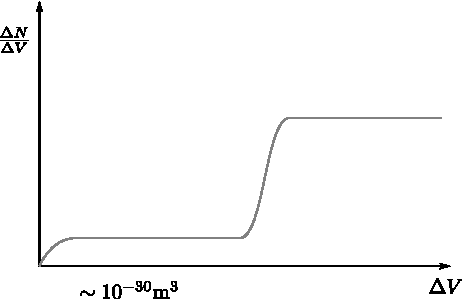
\includegraphics[width=\textwidth]{Plots/patch_centered_not_ink.pdf}
\caption{Density for a patch centered on a point $|\vec{r}|>R$. Here the density is higher for high $\Delta V$, as in these cases the patch comprises also the ink's initial distribution ($\rho_0$).}
\end{figure}
\end{minipage}
%plots
\end{enumerate}
The task is now to compute $\rho(\vec{r},t)$ for $t>0$, given $\rho(\vec{r},0)$.\\
One basic fact, really useful for computing this evolution, is given by the \textit{continuity equation}.\\
The idea is that particles do not move by \q{jumping} between far positions, but travel in a \textit{continuous way}.\\

Consider a box of volume $V$, that contains a fixed number $N$ of particles, with density:
\begin{align*}
N\rho(\vec{r},t) \equiv \rho_n(\vec{r},t)
\end{align*}
Let $A$ be a patch of $V$, with boundary $\partial A$. The number of particles inside $A$ at time $t$ is given by:
\begin{align}
\int_A d^3r \rho_n(\vec{r},t) &= N_A(t)
\label{eqn:N-A}
\intertext{And at later time $t+\Delta t$:}
\int_A d^3r\rho_n(\vec{r},t+\Delta t) &= N_A(t+\Delta t)
\label{eqn:N-A-deltat}
\end{align}
Let's introduce a new quantity, the \textit{current} $\vec{j}(\vec{r},t)$ at position $\vec{r}$ and time $t$. 
Consider a small area $dS$ centered on $\vec{r}$, with normal $\hat{n}$. The number of particles flowing through $dS$ during an interval $\Delta t$ is:
\begin{align*}
\Delta t \vec{j}(\vec{r},t) \cdot \hat{n} dS
\end{align*}
and this can be used to define $\vec{j}$.\\
For example, for a uniform flow of particles with density $\rho_n$ and velocity $\vec{v}$, the \textit{current} is $\vec{j} = \rho_n \vec{v}$.\\

Returning to the problem, we note that the \textit{change} of $N_A$ over time is explained by a flow of particles through the boundary $\partial A$:
\begin{align}
N_A(t+\Delta t) - N_A(t) = - \int_{\partial A} dS \hat{n}\cdot \vec{j}(\vec{r},t)\Delta t
\label{eqn:change-N}
\end{align}
Here we define, by convention, the sign of $\vec{j}(\vec{r},t)$ to be positive if the current is \textit{outward}, that is from $A$ to $V\setminus A$. So, a positive current means that particles are \textit{leaving} $A$, and this explains the $-$ in (\ref{eqn:change-N}).\\

Substituting (\ref{eqn:N-A}) and (\ref{eqn:N-A-deltat}) in (\ref{eqn:change-N}) we arrive at:
\begin{align*}
\int_A d^3r \frac{1}{\Delta t} \left[\rho_n(\vec{r},t+\Delta t)- \rho_n(\vec{r},t) \right] = -\int_{\partial A} dS \vec{j}(\vec{r},t)\cdot \hat{n}(\vec{r}) \cancel{\Delta t}
\end{align*}
Taking the limit $\Delta t\to 0$:
\begin{align*}
\int_A d^3r \frac{\partial}{\partial t}\rho_n(\vec{r},t) = -\int_{\partial A} dS \hat{n} \cdot \vec{j}(\vec{r},t) \underset{(a)}{=} - \int_A d^3r \vec{\nabla} \cdot \vec{j}(\vec{r},t)
\end{align*}
where in (a) we applied the Gauss divergence theorem.\\
Rearranging:
\begin{align*}
\int_A d^3r [\dot{\rho}_n(\vec{r},t) + \vec{\nabla}\cdot \vec{j}(\vec{r},t)] = 0
\end{align*}
Because $\vec{j}$ and $\dot{\rho}$ are continuous functions, by taking $A$ to be sufficiently large, the integral is $0$ if and only if the integrand is everywhere $0$, that is:
\begin{align}
\dot{\rho}_n (\vec{r},t) + \vec{\nabla} \cdot \vec{j}(\vec{r},t) = 0 \qquad \forall \vec{r}, \forall t
\label{eqn:continuity}
\end{align} 
That is the \textbf{continuity equation} in differential form.\\

If there are no fields (EM, gravity, etc.), but we observe a $\vec{j}$, where could possibly be from?\\
The only other relevant physical vector, in this situation, is the \q{spatial} rate of change of density, i.e. its gradient $\vec{\nabla}\rho_n$. In fact, it is observed that particles tend to move \textit{opposite} to the gradient - from regions where there are more particles to regions where there are less. This can be summarized by the \textbf{Fick's Law}:
\begin{align}
\vec{j}(\vec{r},t) = -D\vec{\nabla} \rho_n(\vec{r},t)
\label{eqn:fickslaw}
\end{align}
Of course, there could be some other terms in this expression:
\begin{align*}
\vec{j}(\vec{r},t) = -D\vec{\nabla} \rho_n(\vec{r},t) + C\vec{\nabla}(\vec{\nabla}\rho_n) + \dots
\end{align*}
However, by dimensional analysis, $\partial_x^k \rho_n \sim \rho_n/L^k$, where $L$ is the macroscopic dimension of the container. So, the following terms can be considered negligible.\\

Substituting (\ref{eqn:fickslaw}) in (\ref{eqn:continuity}) we arrive finally at:
\begin{align}
\dot{\rho}_n(\vec{r},t) = \vec{\nabla}(D \cdot \vec{\nabla}\rho_n(\vec{r},t))
\label{eqn:evolution}
\end{align}

Knowing the initial density $\rho_n(\vec{r},0)$, we can know compute the density after a small interval $\Delta t$. For example, we can start by expanding $\rho_n(\vec{r},\Delta t)$ around $\Delta t = 0$:
\begin{align*}
\rho_n(\vec{r},\Delta t) = \rho_n(\vec{r},0) + \Delta t\dot{\rho}_n(\vec{r},0) + O(\Delta t^2)
\end{align*}
Ignoring the higher order terms, we can use (\ref{eqn:evolution}) and compute $\rho_n(\vec{r},\Delta t)$.\\

This maybe more or less doable depending on the form of $D$, that can depend on both $\vec{r}$ and $t$.\\
The $\vec{r}$-dependence is characteristic of problems that are not translational invariant (e.g. a crystal). In fact, if $D$ \textbf{does not} depend on $\vec{r}$, the following holds:
\begin{align*}
\rho(\vec{r},t) = \rho(\vec{r}+\vec{R},t)
\end{align*}
as:
\begin{align}
\dot{\rho}(\vec{r},t) = D\nabla^2 \rho(\vec{r},t)
\label{eqn:evolution-simple}
\end{align}

Note that all the details about the diffusing fluid (e.g. the ink in the previous example) are contained in $D$.\\

Also (\ref{eqn:evolution-simple}) is quite similar to the Schr\"odinger equation for a free particle:
\begin{align*}
\hlc{ForestGreen}{-i} \partial_t \psi = +\hlc{Yellow}{\frac{\hbar}{2m}\nabla^2} \psi
\end{align*}
The yellow term is analogous to $D$, and the only difference is given by the green term. This can be solved by a substitution $\tau = it$ (passing to \q{imaginary time}).\\

Consider the simplest case of a single particle moving in one dimension, with $D$ constant. Let $\rho(x,0) = \delta (x)$. Starting with:
\begin{align*}
\dot{\rho}(x,t) = D\rho''(x,t)
\end{align*}
We define the expected position and velocity values as:
\begin{align*}
\langle x\rangle_t = \int_{-\infty}^{+\infty} \rho(x,t) x\,dx \qquad \frac{d\langle x\rangle_t}{dt} = \int_{-\infty}^{+\infty} \dot{\rho}(x,t)x\,dx
\end{align*}
Using the normalization condition:
\begin{align*}
\int \rho(x,t) dx = 1
\end{align*}
we note that $\rho(\pm \infty,t) = 0$, and also $\rho'(x,t) \to 0$ for $|x|\to \infty$ (otherwise, the density diverges).\\
Then we can solve the problem by subsequent integrations:
\begin{align*}
\frac{d\langle x\rangle_t}{dt} = \int_{-\infty}^{+\infty} \dot{\rho} x\,dx = D\int \rho''x\,dx = D \int \rho\underbrace{\left(\frac{d^2}{dx^2}x\right)}_{=0}dx = 0
\end{align*}
and so:
\begin{align*}
\langle x\rangle_t &= \langle x\rangle_{t=0} = \int dx\, x \rho(x,0) = 0\\
\langle x^2\rangle_0 &= \int dx\,\delta(x)x^2 = 0\\
\langle x^2\rangle_t = 2Dt + \langle x^2 \rangle_0 =\ 2Dt
\end{align*}
\begin{align*}
\frac{d}{dt} \langle x^2 \rangle_t = \int \dot{\rho} x^2 dx = D \int \rho'' x^2 dx =\ D \int \rho(x,t) \frac{d^2}{dx^2}x^2 dx = 2D
\end{align*}
\marginpar{This last part needs some work}
\end{document}


